The elliptic billiard is a particle moving with constant velocity in the interior of an ellipse, undergoing elastic collisions against its boundary \cite{rozikov2018,sergei91}; see Figure~\ref{fig:billiard-trajectories}. It satisfies two integrals of motion: (i) energy: constant velocity and elastic collisions, and (ii) Joachimsthal's: all trajectory segments are tangent to a virtual, confocal ellipse known as the {\em caustic} \cite{sergei91}. The confocal pair renders the elliptic billiard a special case of {\em Poncelet's porism} \cite{dragovic11}: if one $N$-periodic {\em orbit} (a closed trajectory) can be found departing from some boundary point, any other such point can initiate such an orbit, i.e., a 1-dimensional {\em family} of $N$-periodic orbits exists. Integrability produces a first magical consequence: their perimeter is invariant \cite{sergei91}. 

\begin{figure}[H]
    \centering
    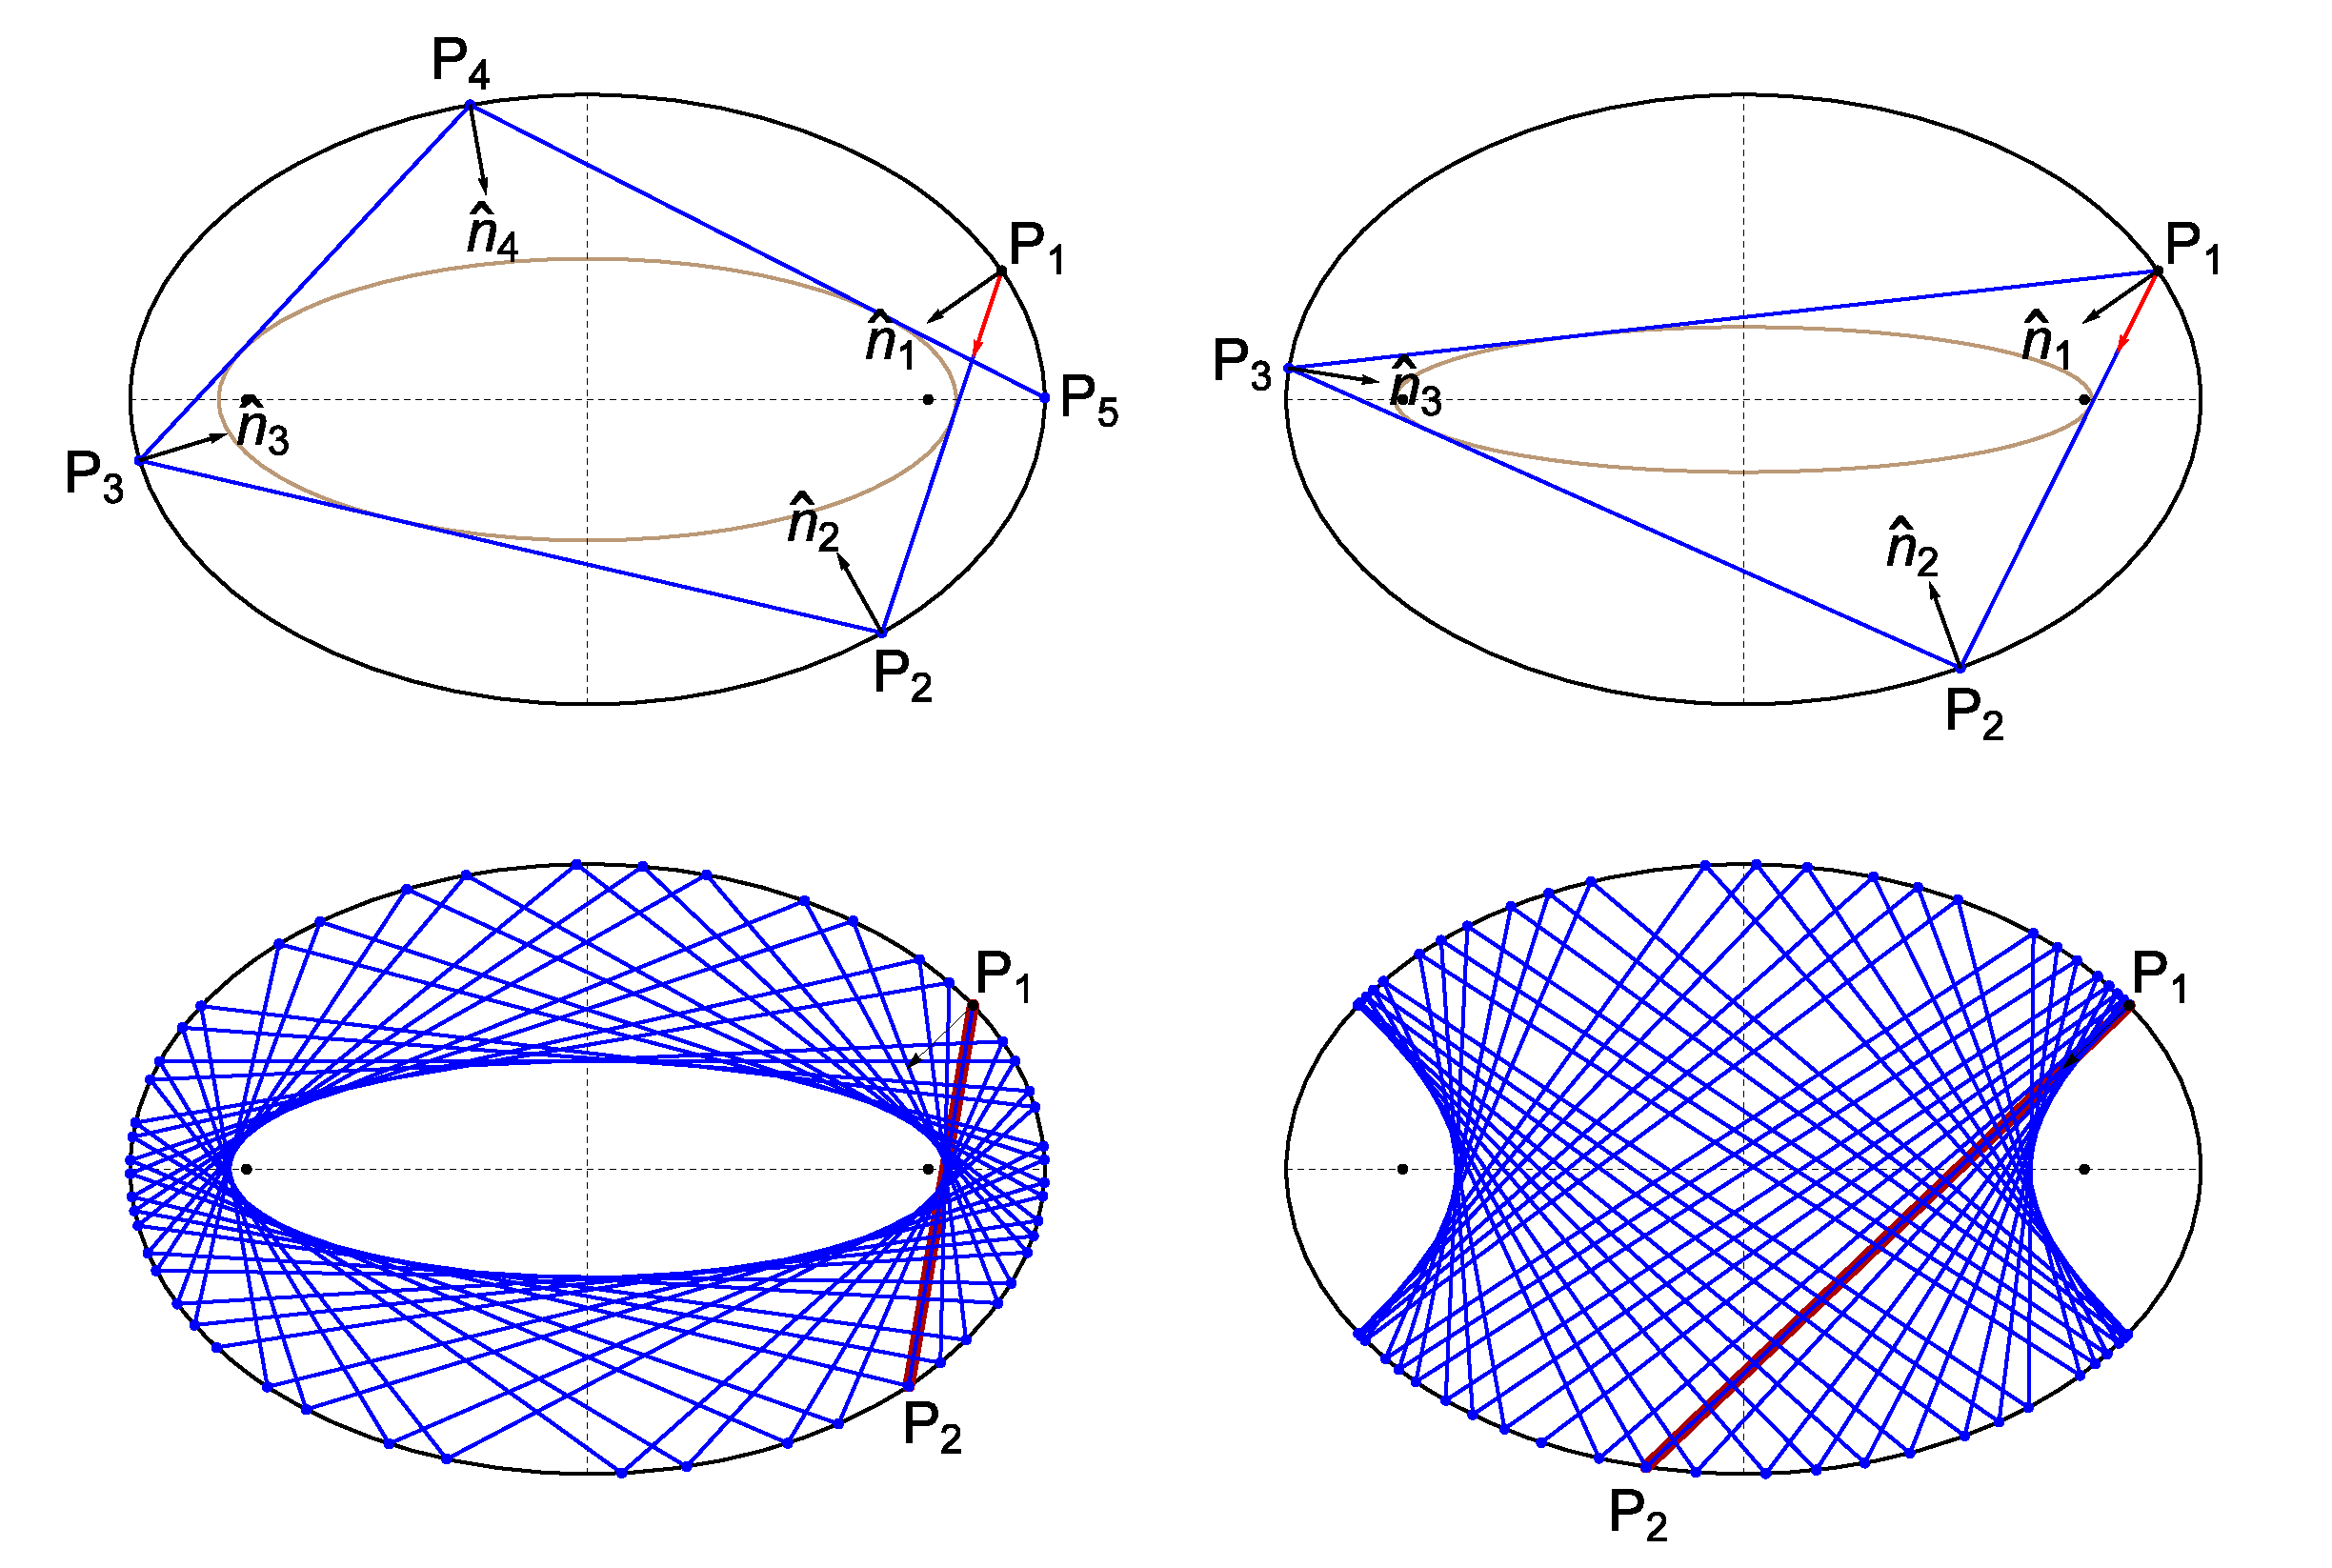
\includegraphics[width=.8\textwidth]{1010_billiard_trajectories.eps}
    \caption{Trajectory regimes in an elliptic billiard. \textbf{Top left}: The first four segments of a trajectory departing at $P_1$ and moving toward $P_2$, bouncing at $P_i, i=2,3,4$. At each bounce the normal $\hat{n}_i$ bisects incoming and outgoing segments. Joachimsthal's integral \cite{sergei91} means all segments are tangent to a confocal {\em caustic} (brown). \textbf{Top right}: All 3-periodic orbits are tangent to a confocal caustic (brown). \textbf{Bottom}: The first 50 segments of a non-periodic trajectory starting at $P_1$ and directed toward $P_2$. Segments are tangent to a confocal ellipse (left) or hyperbola (right). The former (respectively, latter) occurs if $P_1P_2$ passes outside (respectively, between) the elliptic billiard's foci (black dots).}
    \label{fig:billiard-trajectories}
\end{figure}

Here we focus on invariants of 3-periodic orbits; see Figure~\ref{fig:three-orbits-proof}. Because these  are triangles, we make use of an array of classic properties. In \cite{reznik2019-intelligencer,reznik2020-loci} we analyzed the loci of {\em triangle centers} \cite{kimberling97-major-centers} such as the incenter, barycenter, etc. These yield a smorgasbord of algebraic curves: circles, ellipses, quartics, and higher order; see \cite{reznik2019-locus-gallery}.

One early observation was that the locus of the incenter (where bisectors meet) is an ellipse \cite[PL\#01]{reznik2020-playlist-proofs}. Proofs soon followed for the ellipticity of the incenter \cite{olga14}, barycenter \cite{sergei07_grid} and circumcenter \cite{corentin19,garcia2019-ellipses}, and more recently \cite{reznik2020-loci} for 29 out of the first 100 entries in Kimberling's copious Encyclopedia of Triangle Centers (ETC) \cite{etc}, where centers are identified as $X_i$, e.g., $X_1,X_2,X_3$ for incenter, barycenter, circumcenter.

\begin{figure}[H]
    \centering
    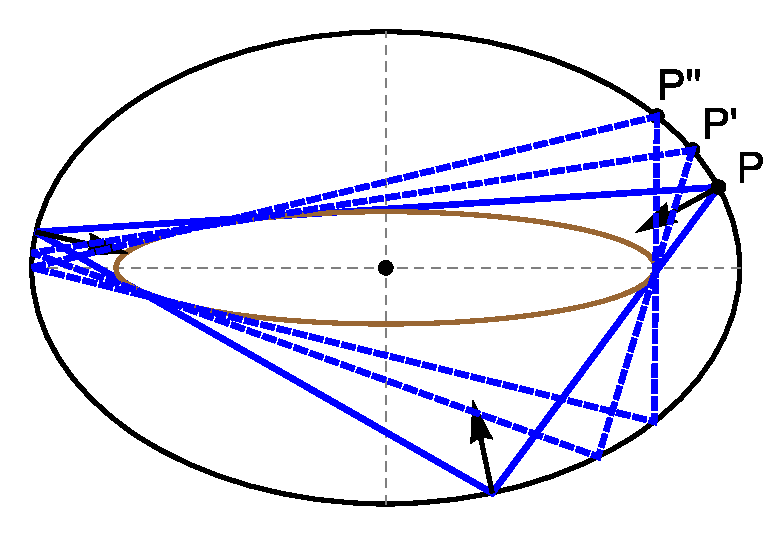
\includegraphics[width=.5\textwidth]{1020_three_orbits_proofs}
    \caption{Three members (blue) of the one-dimensional family of 3-periodic orbits. These are triangles inscribed in an ellipse, whose vertices are bisected by the local normals. Joachimsthal's integral \cite{sergei91} prescribes that all trajectory segments (closed or not) are tangent to a confocal caustic (brown), i.e., this is a special case of Poncelet's porism \cite{dragovic88}. Moreover, the entire family of 3-periodics is tangent to that {\em same} caustic!}
    \label{fig:three-orbits-proof}
\end{figure}

Another interesting observation was that the {\em Mittenpunkt} $X_9$ (where lines drawn from each excenter through sides' midpoints concur \cite[Mittenpunkt]{mw}) is stationary at the billiard center \cite{reznik2019-intelligencer}; see \cite[PL\#02]{reznik2020-playlist-proofs}. \\

\subsection{Main Results.}

\begin{itemize}
    \item Theorem~\ref{thm:rovR}: The 3-periodic family conserves the ratio of inradius-to-circumradius, resulting in several corollaries;
    \item Theorem~\ref{thm:area-ratio-outer-inner}: Invariant area ratio between the 3-periodic orbits' excentral and orthic triangles.
    \item Theorem~\ref{thm:delta-power}: The power of the circumcircle of 3-periodic orbits with respect to the center of the elliptic billiard is invariant.
    \item Theorem~\ref{thm:cosine-circle}: 
    The cosine circle of the excentral triangle to 3-periodic orbits is stationary, centered on the Mittenpunkt, and exterior to the elliptic billiard.
    \item Theorem~\ref{thm:rovR-explicit}: An expression is derived for the invariant inradius-to-circumradius ratio in terms of the two classic invariants of the elliptic billiard (perimeter and Joachmisthal's constant).
\end{itemize}

\bigskip
\subsection{Related Work.}
Examples of triangle families under certain constraints which have been studied include the following: (i) Poristic triangles \cite{Gallatly1913}, with fixed incircle and circumcircle. These by definition   preserve  $r/R$ (an invariant shared with 3-periodics in the elliptic billiard). First studied by Chapple in 1761, then Euler, a modern treatment is given in \cite{Weaver1924,Weaver1933} and \cite{Murnaghan1925}. More recently, several of its triangle centers have been shown to produce circular and pointwise loci \cite{Odenhal2011}, and to be related to the billiard 3-periodics under a similarity transform \cite{garcia2020-poristics}. (ii) Common incircle and centroid: vertices lie on a conic \cite{Pamfilos2011}. (iii)
Triangles with sides tangent to a circle \cite{Nikolina-families2012}. (iv) Triangles associated with two lines and a point not on them \cite{Sliepcevic2013}. Also related is the family of rectangles inscribed in smooth curves \cite{schwartz2018-rectangles}. The locus of centroids of Poncelet polygons is studied in \cite{schwartz2016-com}, whereas that of the circumcenter is studied in \cite{ana2020}.

\bigskip
\subsection{Outline of the article.} In Section~\ref{sec:prelim} we introduce preliminaries. Section~\ref{sec:rovr} contains proofs for invariant inradius-to-circumradius ratio and corollaries. Section~\ref{sec:cosine-circle} describes a stationary circle associated with 3-periodic orbits. Generalizations for $N>3$ appear in Section~\ref{sec:gener}. Section~\ref{sec:experimental} presents experimental results which served as a guide to the theorems. A table of videos illustrating some of the phenomena discussed herein is provided in Appendix~\ref{app:videos} and Appendix~\ref{app:orbit-vertices} provides explicit expressions for 3-periodic orbit vertices.